

\begin{table}[t]
    \scriptsize
	\renewcommand{\arraystretch}{0.5}
	\renewcommand{\theadgape}{\Gape[.2pt]}
% 
%   	\renewcommand\theadfont{\bfseries}

 	\centering
    \begin{subtable}{\columnwidth}
    
 	    \centering
% 	\begin{adjustbox}{width=.9\columnwidth}
		\begin{tabular}{p{20mm}p{55mm}}
    		\toprule
			\multicolumn{2}{c}{\thead{Host Configuration}}\\ 
            \midrule
			\thead{Processor} &  \makecell[l]{8 in-order ARMv7 cores \\ (2 threads/core, clock rate $4.0$ GHz)}\\
			\midrule
			\thead{L1 Cache}  & Per-core, $32$ KB I-cache, $64$ KB D-cache \\
			\midrule
			\thead{L2 Cache}  & Shared across cores, $256$ KB\\  
% 			\hline
            \midrule
			\thead{OS} & Linux kernel 3.16.0-rc6 \\
			
			\bottomrule
% 			% \renewcommand{\arraystretch}{0.1}
% 			% \multicolumn{2}{c}{}\\«
		\end{tabular}
	\end{subtable}
% 	\end{adjustbox}
 	\rule{0pt}{1ex}
%  	\vspace{1mm}
% 	\newline
% 	\begin{adjustbox}{width=.9\columnwidth}
    \begin{subtable}{\columnwidth}
 	\centering
		\begin{tabular}{p{20mm}p{55mm}}
		    \toprule
			\multicolumn{2}{c}{\thead{PIM-enabled Memory Configuration}}\\
		    \midrule	
			\thead{Memory Banks} & \makecell[l]{8 PIM-enabled memory banks, $64$ MB/bank, \\Memory type: \texttt{gem5} \texttt{HMCVault}}  \\
			\midrule
			\thead{PIM Core}  & \makecell[l]{1 $\times$ in-order ARMv7 core per bank \\(1 thread/core, clock rate $1$ GHz) }                           \\
			\midrule
			\thead{Local memory} & $1$ MB per core\\
			\bottomrule
		\end{tabular}
		
    \end{subtable}
% 	\end{adjustbox}
% 	\vspace{1mm}
% 	\newline \begin{adjustbox}{width=1\columnwidth}
% 		\begin{tabular}{p{20mm}p{60mm}}
% 			\toprule
% 			\multicolumn{2}{c}{\bfseries DRAM Configuration}                        \\
%             \midrule
% 			\bfseries DRAM parameters & Row buffer size: 256B, burst size: 32B
% 			tRP: 13.75ns, tRCD: 13.75ns, tCL: 13.75ns, tBURST: 3.2ns                    \\
%         	\bottomrule
% 		\end{tabular}
% 	\end{adjustbox}
	\caption{Configuration of the simulated system.}
	\label{table:config}
\end{table} 

\begin{figure*}[t]
  \centering
  \begin{subfigure}{.8\textwidth}
  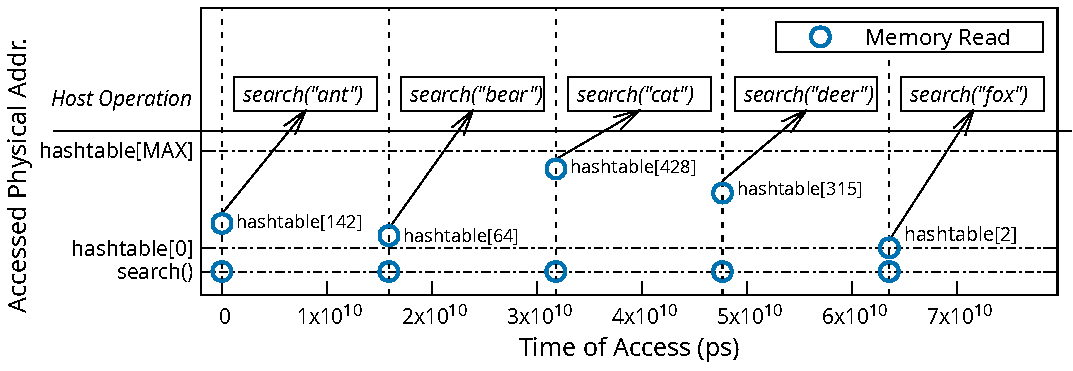
\includegraphics[width=.975\columnwidth]{figures/sepim/host-access-pattern.pdf}
  \caption{Memory access pattern observed on memory bus during host enclave dictionary lookup.}
  \label{fig:host-pattern}
  \end{subfigure}
\begin{subfigure}{.8\textwidth}
  \centering
  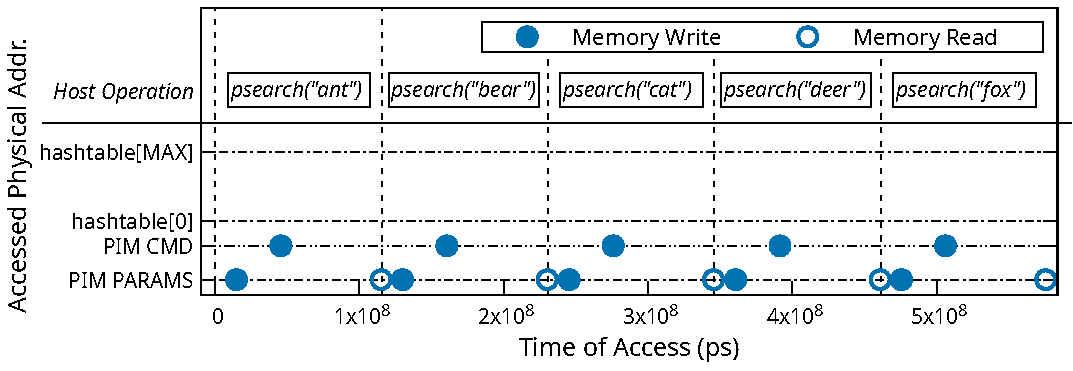
\includegraphics[width=.975\columnwidth]{figures/sepim/pim-access-pattern.pdf}
  \caption{Memory access pattern observed on the memory bus during \thename-assisted dictionary lookup.}
  \label{fig:pim-pattern}
  \end{subfigure}
  \caption{Memory access pattern observed on bus during confidential \texttt{hunspell} dictionary program. In host CPU enclave-only model, accessed \texttt{hashtable} location reveals  looked up word. In \thename-assisted model, observed memory pattern is consistent for all looked up words.}
  \label{fig:access-pattern}
\end{figure*}

\section{Evaluation}


%\fix{Do we evaluate robustness against side-channels?}
We evaluated \thename through a cycle-accurate simulation. The simulation configuration we used for simulating our system can be found in \autoref{table:config}. Note that we assume the presence of processor enclaves in the host, as our simulator does not support simulation of enclaves such as SGX~\cite{sgx} or TrustZone~\cite{arm-tz}. We assume that \thename cooperates with the host enclave to achieve confidential computation. For this reason, we did not consider the overhead from the use of host processor enclaves, although the exclusion of the overhead works against our favor. We configured the PIM core to operate at the clock rate of $1$ GHz to reflect the power and area constraint in the DRAM or 3D-stacked memory packages. The timing parameters used for the simulation were determined through existing works that conducted simulations on similar hardware~\cite{smcsim,concurrent-data,tesseract}. There are 8 \thename-enabled memory banks inside the memory module that can execute independently. We take advantage of all 8 \thename-enabled memory banks in the data-intensive performance evaluation in \cref{subsec:app-perf}. Other benchmarks use only a single memory bank.

Our evaluations show vital aspects of our design: first, we show that offloading computations to \thename leak no address-based side-channels on the bus. Second, we show that our introduced modifications do not inhibit PIM's ability to perform data-intensive computation efficiently. Finally, we also demonstrate \thename's benefits as enclave extended memory. We first show the lack of bus traffic side-channel in \cref{subsect:memory-access-pattern}. We perform a set of microbenchmarks to evaluate the performance of encrypted data movement and the secure memory access interface in \cref{subsec:microbench}. Lastly, we evaluate the data-intensive computation performance of \thename-assisted confidential k-mean clustering application in \cref{subsec:app-perf}.

%We first provide a security analysis of \thename against the \fix{attack vectors that exist in our threat model in \cref{subsec:sec-analysis}}. 







\subsection{Memory Access Pattern Analysis}
\label{subsect:memory-access-pattern}
\begin{figure}[h]
    \centering
    \begin{minted}{c}
struct data_item *search(const char* key) {
    int index = murmur3_hash(key) % TABLE_SIZE;
    while (hashtable[index].value != -1) {
        if(key_match(hashtable[index], key))
            return &hash_array[index];
        ++index;
        index %= TABLE_SIZE;
    }
    /* Key not found */
    return NULL;
}
\end{minted}
\caption{Dictionary word lookup function used for memory access pattern analysis.}  
\label{lst:search}
\end{figure}


% w{We conduct a memory access pattern analysis to demonstrate that by offloading the operations on data structures to \thename, memory trace obliviousness can be achieved.}
We set up an experiment that imitates the off-chip bus snooping attack illustrated in Membuster~\cite{membuster}. The attack demonstrates that bus snooping can undermine the confidentiality of processor enclaves through memory access pattern analysis on the bus traffic. Our test program is a minimal hash table lookup that mimics the attack examples on the \texttt{hunspell} dictionary program shown in Membuster. Each entry in the hash table stores a hash key and an integer value in the place of the word's definition for simplicity. The attack illustates how the address side channel observable on the bus can reveal the behavior of the seemingly protected computation. We implemented a \texttt{search()} function that takes a string as an argument. The argument is hashed using the \emph{Murmur3} hash algorithm, then used as an index to the hash table. The exact operation of \texttt{search()} is defined in \autoref{lst:search}.


\begin{figure*}[t]
  \centering
  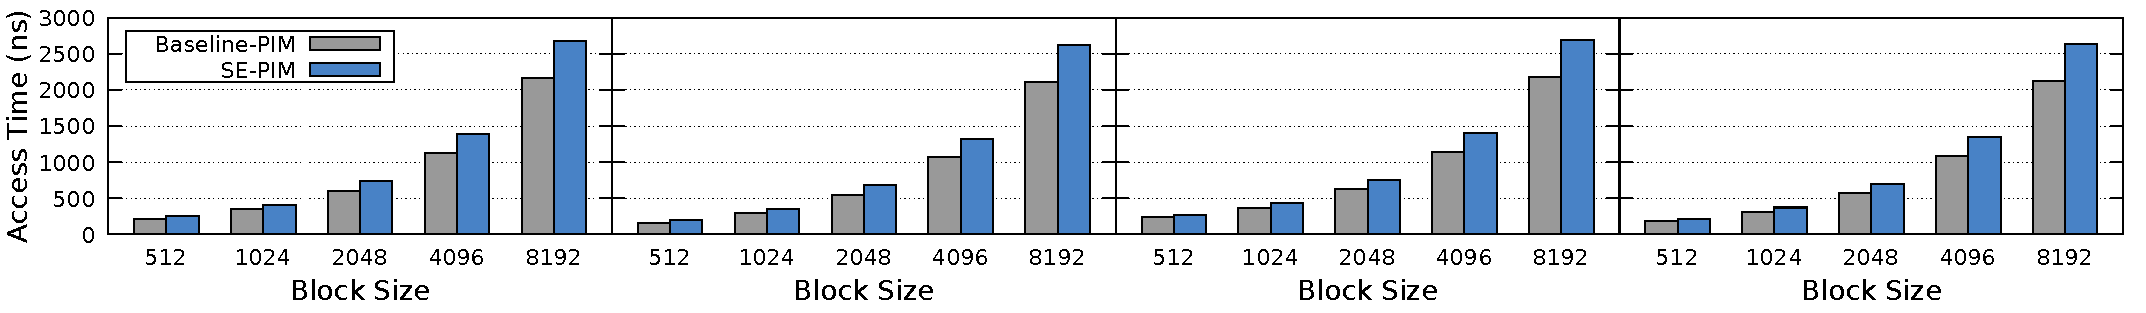
\includegraphics[width=0.95\linewidth]{figures/sepim/pim-microbenchs.pdf}
  \begin{subfigure}{.23\textwidth}
  \caption{Sequential read}
    \end{subfigure}%
  \begin{subfigure}{.23\textwidth}
  \centering
%   \includegraphics[width=0.95\linewidth]{data/gnuplot/pim-seq-write.pdf}
  \caption{Sequential write}
    \end{subfigure}%
  \begin{subfigure}{.23\textwidth}
  \centering
%   \includegraphics[width=0.95\linewidth]{data/gnuplot/pim-rand-read.pdf}
  \caption{Random read}
\end{subfigure}%
  \begin{subfigure}{.23\textwidth}
  \centering
%   \includegraphics[width=0.95\linewidth]{data/gnuplot/pim-rand-write.pdf}
  \caption{Random write}
\end{subfigure}%
\caption{Access latency of AES-encrypted DMA from bank memory to PIM local memory of \thename vs. Baseline-PIM without encryption.}
\label{fig:dma-latency}
\end{figure*}

The original attack from~\cite{membuster} requires that the host enclave caches are constantly flushed to yield reliable and distinct access patterns on the bus. We adapted the same premise for our experiment. However, since the gem5 x86 CPU model does not correctly simulate the cache flush instructions (e.g., \texttt{clflush}), we implemented a function that forces cache flush by repetitive memory accesses and used it after each hash table access to preventing caching. In the host-only setup, which represents a case where the host processor enclave is used to protect the hash table, we place the hash table inside a single memory page so that it is contiguous in physical memory. Then, we obtain the virtual to physical mapping of the program from \texttt{/proc/\{process pid\}/pagemap}. For the PIM-assisted version of the program, the hash table is stored in the PIM memory bank, and a PIM kernel that performs hash table lookups is loaded into the PIM processor local memory. We leverage our simulation framework to place a memory tracing unit between the L2 cache and DRAM (i.e., the memory bus) to collect the accessed physical addresses. \autoref{fig:access-pattern} illustrates the memory access pattern observed on the bus -- by the attacker who is snooping on the bus traffic -- in host processor execution and \thename-assisted execution.
\autoref{fig:host-pattern} shows the memory access pattern recorded during the execution of the host-only version of the test program, and \autoref{fig:pim-pattern} shows that of the \thename-assisted version (\texttt{psearch()}). The memory writes are denoted by \textcolor{blue}{$\bullet$} and reads by \textcolor{blue}{$\circ$}. 

\hdr{Results.} 
%\hjc{If you are going to use this hdr, do it for all experiments}
In the CPU-only version, the executed function and the words looked up in the hash tables are observable to the adversary. With the assumption that the adversary has the pre-obtained knowledge on the addresses of the functions and data of the program, the adversary learns that \texttt{search()} has been executed and in-memory dictionary locations, such as \texttt{hashtable[7]}, \texttt{hashtable[237]}  are accessed. As a result, the adversary can eventually infer the queried words by looking at the bus traffic. On the other hand, the PIM-assisted version shows only the communication with PIM. The PIM command channel and parameter channel are fixed single-channel memory-mapped I/O channels. The host program first writes the parameter (e.g., \texttt{"apple"} to the parameter channel, then writes the command number that corresponds to the PIM function \texttt{search()} in the PIM kernel to the command channel to invoke the offloaded task. These patterns are identical to all PIM kernel invocation, regardless of the invoked function and parameters. Also, data access (e.g., the hash table in this example) is contained inside the DRAM package. This example clearly shows the security advantages of \thename against side-channel attacks that target the bus traffic. We further discuss the security of \thename in a more comprehensive manner in \cref{sec:discussion}.






\subsection{Microbenchmarks}
\label{subsect:aes-dma}
\label{subsec:microbench}
We measure the performance of encrypted DMA transfer and the secure memory access interface with our microbenchmarks. The results suggest that encrypted DMA transfer would incur only minor overhead in each transfer, and the throughput of the controlled memory access channel would scale with the transfer size.

%Second, we measure the throughput of the memory accesses performed by host enclave through the secure access interface (explained in \cref{subsec:secure-access}). 

% We measure the performance of two operations, the encrypted data movement between PIM local memory and the memory bank, and


% Encrypted data movement is the fundamental building block of \thename design. PIM core accesses data in the memory bank by decrypting and moving the encrypted data into its local memory. . We evaluated the performance of encrypted data movement using \thename simulation to measure its performance. In the experiment, the access times and throughput of AES-enabled DMA transfers in a single \pimenclave are measured and compared with the baseline PIM simulation model, which we shall call \emph{PIM-Baseline}, that does not support any cryptographic protection for DMA transfers.







\subsubsection{Encrypted DMA transfers}
We evaluate the overhead of encrypted data movement between PIM local memory and the memory bank, when accelerated by the hardware AES engine. The average throughput of the operation is also evaluated. For both PIM-baseline and \thename, we measured the access time for the following cases: 1. in both directions (local-to-bank and bank-to-local), 2. sequential and random accesses and 3. for varying block sizes.

\hdr{Results.}  \autoref{fig:dma-latency} illustrates the average access time measured for $1000$ DMA accesses in each configuration. The access time for random and sequential access is roughly similar because there is no cache on PIM that incurs variations in access time. Our simulation results report an average of $22.35$\% of increase in access time due to the AES-capable DMA engine. This is in line with the previous works that simulated the performance overhead of hardware AES support, such as~\cite{obfusmem,invisimem}. 

We further investigated the throughput for data transfer between the memory bank and local memory. The DMA maximum throughput of moving data with the AES-capable DMA engine is compared to that of without encryption in PIM-Baseline. Overall, the AES-enabled DMA engine produces an average throughput of $2.9$ GB/s, compared to $3.53$ GB/s for unencrypted DMA accesses.
\begin{figure}[t]
    \centering
    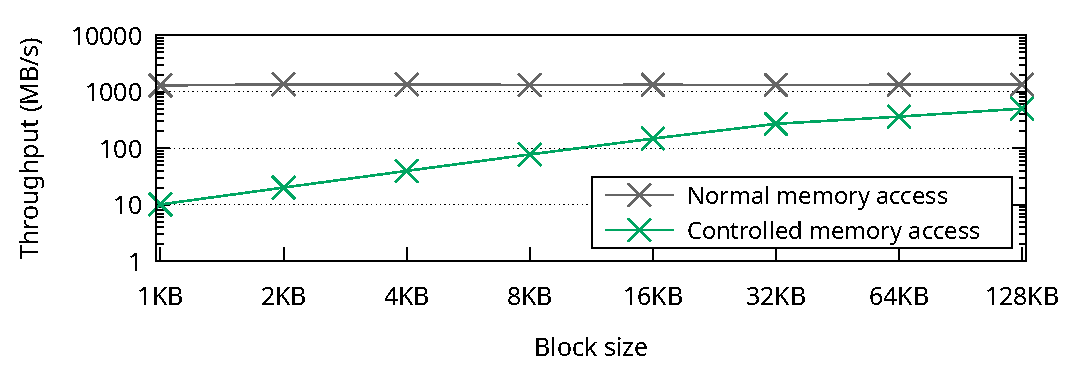
\includegraphics[width=.80\textwidth]{figures/sepim/secure-interface-throughput.pdf}
    \caption{The throughput of the controlled memory access channel on different block sizes in log-scale.}
    \label{fig:secure-access-throughput}
\end{figure}


\subsubsection{Controlled data access throughput}
\label{subsec:secure-access-eval}
We measure the throughput of data access performed through the controlled data channel (\cref{subsec:secure-access}) and compare it to the throughput of normal DRAM access to the memory. The throughput of different block sizes are measured. 



\hdr{Results.} \autoref{fig:secure-access-throughput} illustrates the results of the evaluation. Only read accesses are shown, since the performance of read and write accesses is almost identical. The results show that when small block sizes are used, a large proportion of the overhead comes from the communication channels (e.g., the MMIO accesses for writing commands), which significantly degrade the throughput of the controlled memory access channel. For instance, the throughput of $1$ KB block accesses is $127\times$ lower than normal memory accesses. However, the throughput is significantly higher when larger block sizes are used, $362.7$ MB/s for $64$ KB blocks and $504.2$ MB/s for $128$ KB blocks. The throughput of normal memory access is roughly the same among different block sizes, about $1300$ MB/s.
Despite having a lower throughput than direct memory access, the interface is faster than most ORAM implementations, which include expensive reshuffling operations at each memory access~\cite{zerotrace}. Since most of the data is already placed inside memory for PIM computation, we expect the controlled memory accesses not to be a bottleneck in PIM workloads.



%the interface would not become a bottleneck for \thename applications, since most PIM workloads reuse data within the memory bank.
%Since for most PIM workloads, data mostly stays inside memory 


% General algorithm

% \begin{figure}[b]
%   \setlength{\belowcaptionskip}{-10pt}
%   \centering
%   \includegraphics[trim=0 0 0 0,width=\linewidth]{images/bandwidth.eps}
%   \caption{Peak throughput for DMA transfers}
%   \label{fig:dma-bandwidth}
% \end{figure}



% \begin{figure}[b]
%     \centering
%     \includegraphics[width=.8\columnwidth]{images/k-mean.pdf}
%     \caption{The simplified diagram of $k$-mean clustering algorithm between host and \thename. The host send the parameters, including the current global clusters (e.g., $x_G, y_G, z_G$) to command \pimenclaves to start execution. On each \pimenclave, the kernel loop through the data points stored in the memory bank and update the local clusters (e.g., $x_L, y_L, z_L$), until all data points are processed. Then, the \pimenclave send the updated cluster, along with the \emph{delta} value to the host. The host uses information aggregated from \pimenclaves to update the global cluster, then start another round of $k$-mean if needed. }
%     \label{fig:kmean}
% \end{figure}
% \fix{This can be general PIM-enclave computation model? does it need to be a dedicated figure for k-mean?}

\begin{figure*}[t]
%   \setlength{\belowcaptionskip}{-10pt}
  \centering
  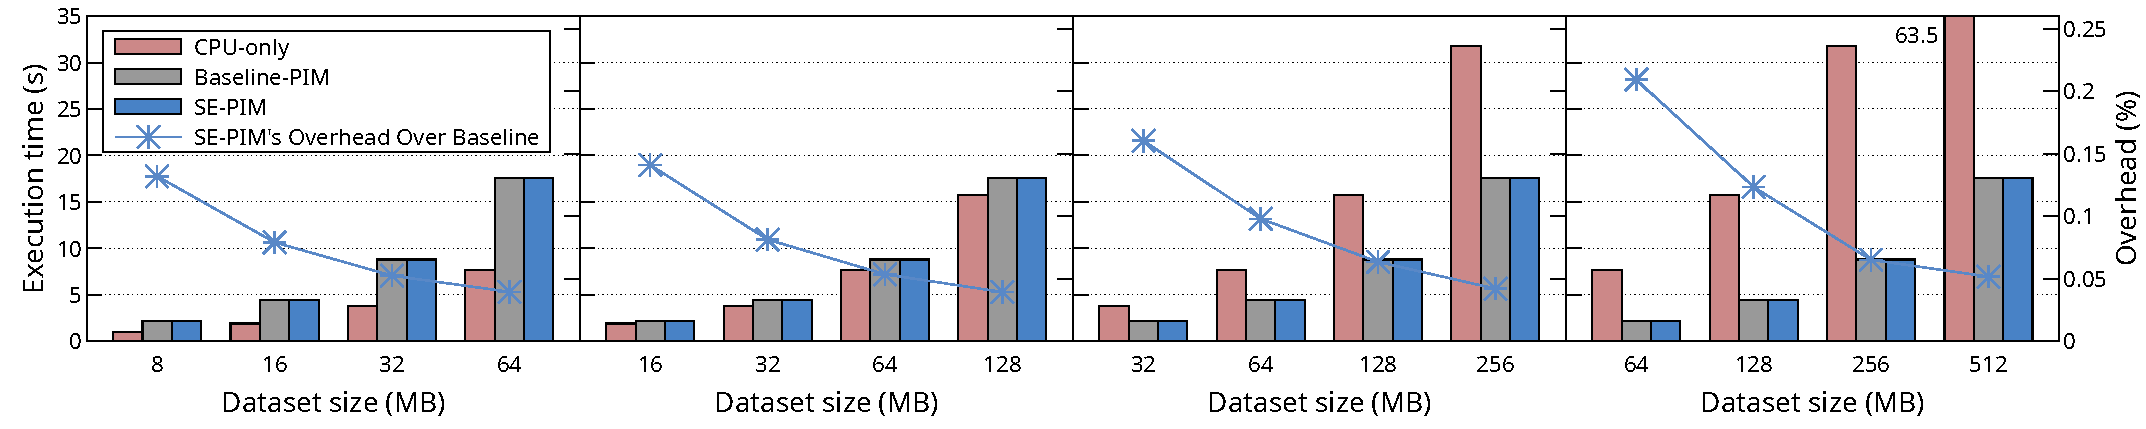
\includegraphics[width=0.95\textwidth]{figures/sepim/kmean-performance.pdf}
    \begin{subfigure}{.23\textwidth}
  \caption{1 PIM Core}
    \end{subfigure}%
  \begin{subfigure}{.23\textwidth}
  \centering
%   \includegraphics[width=0.95\linewidth]{data/gnuplot/pim-seq-write.pdf}
  \caption{2 PIM Cores}
    \end{subfigure}%
  \begin{subfigure}{.23\textwidth}
  \centering
%   \includegraphics[width=0.95\linewidth]{data/gnuplot/pim-rand-read.pdf}
  \caption{4 PIM cores}
\end{subfigure}%
  \begin{subfigure}{.23\textwidth}
  \centering
%   \includegraphics[width=0.95\linewidth]{data/gnuplot/pim-rand-write.pdf}
  \caption{8 PIM Cores}
\end{subfigure}%
  \caption{The execution time of confidential k-mean using \thename against the baseline PIM and CPU-only versions (without data encryption). \thename overhead over the baseline PIM and the performance numbers of using different numbers of PIM cores are measured.}
  \label{fig:kmean-perf-versus-baseline}
\end{figure*}

\subsection{Protected Data-intensive Computation Performance}
 
\label{subsec:app-perf}
\label{subsec:kmean}
% \input{figures/k-mean}
% \new{We developed a proof-of-concept application to evaluate the performance in data-intensive applications and the feasibility of the programming model. We choose $k$-mean as a representative application, because ... . First, it does not require frequent direct data access. Second, the computation can be distribute onto multiple \pimenclaves, which highlight the performance characteristics of PIM~\cite{upmem-atc}}
% \wip


To evaluate the performance of \thename on real-world workloads, we implement a confidential k-mean clustering application powered with \thename and compare its performance with an implementation on the baseline PIM. 
k-mean clustering is a standard algorithm in data analytics that aggregates data points into clusters. The application requires a large amount of data movement, making it a prime candidate for PIM-based accelerator~\cite{dual,prins}. 
In our confidential k-mean clustering, the adversary observing the computation learns no information about the computation. Moreover, our system allows the host enclaves to process data larger than the memory limitation of SGX-based enclaves ($96$ MB). When 8 \thename-enabled memory banks are used, up to $512$ MB of data can be processed concurrently. As more \thename units are employed, more data can be processed. 

%The algorithm starts by selecting a group of $k$ coordinates as the \emph{centroids} of the initial clusters, then iteratively updates the centroids of clusters in two steps. First, it \emph{assign} every data point to their nearest cluster, i.e., the cluster that has the smallest \emph{Euclidean distance} to the data point. Then, it \emph{update} the centroids by finding the mean of data points that belong to a cluster.

% \hdr{Evaluation objective. }



% In our $k$-mean implementation, we offload the core algorithm that incurs frequent memory access to \thename. The host distributes the encrypted data into multiple \thename memory banks, sends commands and parameters to \thename PIMs to initiate computation, then collects and aggregates the results into new \emph{global centroids}.  Upon receiving the command, the $k$-mean PIM kernel is executed in response. The kernel finds \emph{pointer} to the data to be computed in the DMA buffer along with other parameters. 
% How it is implemented as PIM kernel and PIM-enclave specific programming model

% \hdr{Advantages of \thename-assisted k-mean clustering.}
% The k-mean algorithm on \thename demonstrates our capabilities as a large data accelerator and secure storage by the host. In the algorithm, no data movement occurs between the host enclave and PIM between each kernel execution. Instead, only the arguments for the kernel execution, which includes the pointer of data, the size, the initial clusters, are sent from the host enclave to PIM. After a PIM kernel finishes its execution, only computation results are sent back to the host enclave through the secure channel. The elimination of data movement has two significant implications. First, efficiency was achieved in terms of the total execution time of the particular task and memory bus bandwidth usage. Second, the computation did not leave any pattern on the memory bus. This is only possible on PIM-based computation since CPUs, or any accelerators on the peripheral bus, inevitably access memory with patterns unless using ORAM primitives. With DRAM lockdown, our system also eliminates the access pattern leaked by the memory content changes from data update of the membership data~(\cref{subsec:access-control}).

% \thename also function as a secure memory extension for the host enclave. After data have been loaded into the \pimenclaves, the host enclave need not keep the data inside its EPC memory. Our secure memory access interface described in \cref{subsec:secure-access} hides the address side-channel in cases where host-side data accesses are required. Moreover, the more of \thename units are employed, the more data the host enclave can process and use without EPC swapping. This allows us to overcome the memory limitations of CPU-based secure enclaves.

\hdr{Implementation details.} 
We implement k-mean clustering to perform the data aggregation part on \thename and the baseline PIM. A dataset of randomly generated data points with $16$ different coordinates is used. We preprocess the dataset by partitioning data coordinates into $8$ KB blocks. For the \thename version of k-mean, we encrypt batches of data into encrypted blocks. For each data block, we also use a structure to store the \emph{membership data} (e.g., which cluster the objects belong to) of objects in the block and load them along with the objects into the memory bank. When multiple PIM cores are utilized, data is distributed evenly among the memory banks of different PIM cores. We then create a CPU thread for each PIM core to launch the PIM kernel and wait for the results. The host use the \emph{local clusters} aggregated from different PIM banks to update the \emph{global clusters}.

We implement the PIM kernel to perform k-mean aggregation on data inside the memory bank in a batch of $127$ objects at a time. Each processing batch fetches the objects and their membership data inside the bank memory into local memory. First, it assigns every data point to its nearest cluster, i.e., the cluster that has the smallest \emph{Euclidean distance} to the data point. Then, it recalculates the local clusters of data points inside the memory bank. Finally, the kernel encrypts updates the new membership data into memory before moving on to the next batch. In the version of k-mean powered by \thename, data movement between the local memory and the memory banks is automatically encrypted/decrypted by the AES-capable DMA engine (\cref{subsec:aes-dma}). After all data in the memory bank has been processed, the kernel sends the results (the local clusters and additional metadata) to the host.





\hdr{Results. }
\autoref{fig:kmean-perf-versus-baseline} demonstrates the performance of executing a round of k-mean on \thename in comparison to executing the same algorithm on the baseline PIM. For PIM-based scenarios, we repeat the experiment until the maximum capacity of the PIM-enabled memory banks is reached. When 8 PIM cores are used, the maximum size of the data set is $512$ MB, which corresponds to $80,000,000$  data points. We also measure the algorithm's performance on the CPU (without PIM assistance) on similar data sizes for comparison. The specification of the CPU is described in \autoref{table:config}.

The simulation results support that using that \thename as an accelerator for large data secure computation is efficient. 
The total runtime of \thename's confidential k-mean on encrypted data has negligible overhead to the baseline model without encryption. The results also show that as the data set sizes increase, the overhead of \thename over \baseline also decreases. On average, the execution time of the confidential k-mean algorithm incurs $0.075$\%, $0.079$\%, $0.09$\%, $0.11$\% overhead compared to the insecure version when 1, 2, 4, and 8 PIM cores are used, respectively. Moreover, our system attains speed up in execution time compared to performing k-mean only with the CPU. \thename outperforms the CPU-only k-mean when more than 4 PIM cores are used. When processing $512$ MB of data with 8 PIM cores, \thename achieves $3.61 \times$ speed up to just using the CPU, with the execution time of $17.6$ seconds ($0.05$\% more than the baseline-PIM version). Note that the application's execution time on the CPU is optimistic in our evaluation. We do not consider the overhead of EPC swapping due to extensive memory usage, which can incur up to $1000\times$ performance degradation in some applications~\cite{zerotrace,scone}.


% Moreover, the performance of \thename's k-mean scales with the number of PIM cores. This is  %We use increasing dataset sizes up to $64$ MB, which corresponds to $10,000,000$ data points. % When only $4$ \thename PIM devices are deployed, the execution time of $k$-mean is below that of the host on the same amount of data, with $21.7\%$ performance degradation. The reason is that there is a bottleneck in the communication between the host and PIM. However, \thename outperformed the execution time of the host with more than six \thename-enabled PIMs.